% bianca-epfl.tex
\section{Titan aeroshell using imported grids}
\label{titan-aeroshell-sec}
%
Another aeroshell model is shown in Figure\,\ref{bianca-aeroshell-fig}.
The grids were generated by Bianca Capra using ICEM-CFD grid generation
software and written as Plot3D format file.
These files were then converted to VTK files with the following script:

\noindent
\baselineskip=1.0pc
\topbar\\
\begin{verbatim}
#!/bin/sh
# prepare_grid.sh

gzip -d icem_grid_plot3d.fmt
import_grid.py --input=icem_grid_plot3d.fmt \
               --output=icem_grid \
               --plot3dplanes
gzip icem_grid_plot3d.fmt

echo "Done."
\end{verbatim}
\bottombar

\baselineskip=1.5pc
\medskip
The identification of the (seemingly random) orientation of each block
was done manually by loading the VTK data into ParaView and examining the grid
planes as the indices were adjusted from one limit to another.


\begin{figure}[htbp]
\mbox{
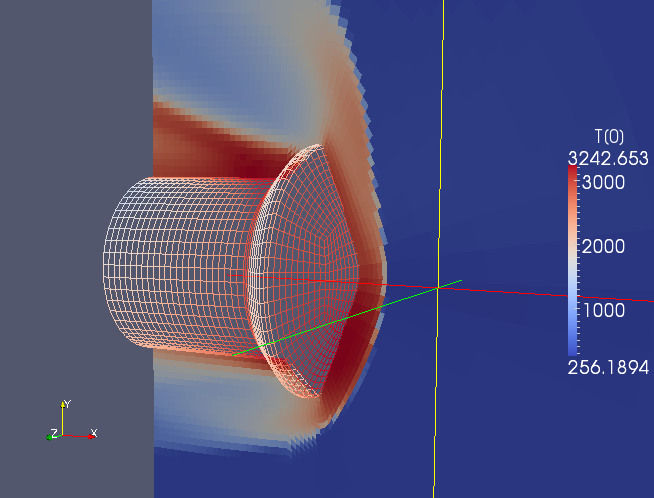
\includegraphics[width=0.5\textwidth]{../3D/bianca-epfl/titan-T-field-with-surface-mesh.png}
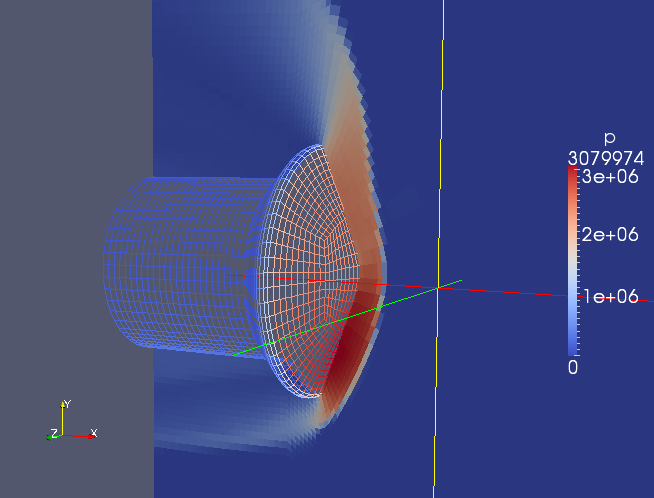
\includegraphics[width=0.5\textwidth]{../3D/bianca-epfl/titan-p-field-with-surface-mesh.png}
}
\caption{Views of the temperature and pressure fields around a Titan aeroshell.
  The surface grid is shown as a wire-frame rendering and a vertical slice (with solid colouring)
  is made through the flow field around the aeroshell.}
\label{bianca-aeroshell-fig}
\end{figure}

\medskip
Once in VTK format, the block meshes can be read in and used as 
\texttt{ParametricVolume} objects within the user's job script.
We can then generate grids of arbitrary resolution from the original ICEM grids.
Note that the bulk of the script is used to assign the boundary conditions 
to each block because the original information about boundary conditions (as
might have been part of the ICEM database) is not available from the Plot3D file.

\medskip
Because this exercise is only to show that complex grids can be imported, the
simulation was run at low grid resolution and to a final time of 300\,ms.
This is long enough for the Mach 7 flow to establish over the aeroshell and,
on the \texttt{geyser} server, took just under one hour (3554\,s) of CPU time 
and required 2251 steps.

\bigskip
\subsection{Input script (.py)}
\index{geometric element!MeshVolume!example of use}
\topbar
\lstinputlisting[language={}]{../3D/bianca-epfl/titan_x2_shell.py}
\bottombar
